

%\documentclass[12pt]{article}
\documentclass[11pt]{scrartcl}
\title{EN2550_Assignment4}
\nonstopmode
%\usepackage[utf-8]{inputenc}
\usepackage{graphicx} % Required for including pictures
\usepackage[figurename=Figure]{caption}
\usepackage{float}    % For tables and other floats
\usepackage{verbatim} % For comments and other
\usepackage{amsmath}  % For math
\usepackage{amssymb}  % For more math
\usepackage{fullpage} % Set margins and place page numbers at bottom center
\usepackage{subcaption}
\usepackage{paralist} % paragraph spacing
\usepackage{listings} % For source code
\usepackage{subfig}   % For subfigures
%\usepackage{physics}  % for simplified dv, and 
\usepackage{enumitem} % useful for itemization
\usepackage{siunitx}  % standardization of si units
\usepackage{hyperref}
\usepackage{tikz,bm} % Useful for drawing plots
%\usepackage{tikz-3dplot}
\usepackage{circuitikz}
\bibliographystyle{IEEEtran}
\usepackage{cite}
\usepackage{mhchem}

%%% Colours used in field vectors and propagation direction
\definecolor{mycolor}{rgb}{1,0.2,0.3}
\definecolor{brightgreen}{rgb}{0.4, 1.0, 0.0}
\definecolor{britishracinggreen}{rgb}{0.0, 0.26, 0.15}
\definecolor{cadmiumgreen}{rgb}{0.0, 0.42, 0.24}
\definecolor{ceruleanblue}{rgb}{0.16, 0.32, 0.75}
\definecolor{darkelectricblue}{rgb}{0.33, 0.41, 0.47}
\definecolor{darkpowderblue}{rgb}{0.0, 0.2, 0.6}
\definecolor{darktangerine}{rgb}{1.0, 0.66, 0.07}
\definecolor{emerald}{rgb}{0.31, 0.78, 0.47}
\definecolor{palatinatepurple}{rgb}{0.41, 0.16, 0.38}
\definecolor{pastelviolet}{rgb}{0.8, 0.6, 0.79}
\newcommand{\SubItem}[1]{
    {\setlength\itemindent{15pt} \item[-] #1}
}
\begin{document}

\begin{center}
	\hrule
	\vspace{.4cm}
	{\textbf { \large Stellar Evolution and Galaxies}}
\end{center}
{\textbf{Student Name:}\ Nuwan Bandara \hspace{\fill} \textbf{Submitted Date:} September 3, 2021   \\
{ \textbf{Institute:}} \ Institute of Astronomy, Sri Lanka \hspace{\fill} \textbf{Assignment Number:} 2 \\
	\hrule

\bigskip

\paragraph*{Problem 1} %\hfill \newline
\begin{enumerate}[label=(\alph*)]
\item Both the pp-chain and the CNO-cycle produce energy via a set of reactions (which we studied in the lectures). Both of these reactions are important during the main-sequence evolution of stars. What is practically the difference between the pp-chain and the CNO-cycle?
\newline \textbf{Answer: }
\newline The CNO cycle differs from the pp-chain since,
\begin{itemize}[noitemsep,nolistsep]
%\itemsep-1em
    \item  CNO-cycle needs carbon to be present to act as a catalyst
    \item CNO-cycle is more temperature dependant than pp-chain to overcome the strong Coulomb barrier
    \item pp-chain has three simultaneous branches while CNO-cycle has two branches each with six reactions 
\end{itemize}
\item When investigating the stellar structure, which parameters are important?
\newline \textbf{Answer: }
\begin{itemize}[noitemsep,nolistsep]
%\itemsep-1em
    \item (Initial) mass
    \item Composition (especially the metallicity)
    \item Rotation rate 
\end{itemize}
\item If the sun were to collapse into a neutron star with a radius of 8 km, what would be its density? (Assume no mass loss)
\newline \textbf{Answer: }
\newline Since there is no mass loss and assuming the sun and the neutron star as perfect symmetrical spheres,
\begin{equation}
    \frac{4\pi R^3_\odot \rho_\odot(r)}{3} = \frac{4\pi R^3_\star \rho_\star(r)}{3}
\end{equation}
\begin{equation}
    \rho_\star(r) = \frac{R^3_\odot \rho_\odot(r)}{R^3_\star} = \frac{696340^3 \times 1400}{8^3}= 9.233 \times 10^{17} kgm^{-3}
\end{equation}
\item The escape velocity of an object is given as $v_{esc} = \sqrt{\frac{2GM}{R}}$. If the sun were to turn into a black hole
(without any mass loss), how small would it need to be?
\newline \textbf{Answer: }
\newline If the sun were to turn into a black hole, then the escape velocity should be at least the velocity of light (in a vacuum). Therefore, 
\begin{equation}
    c = \sqrt{\frac{2GM}{R_S}} \rightarrow R_S = \frac{2GM}{c^2}
\end{equation}
\begin{equation}
    R_S = \frac{2 \times 6.67 \times 10^{-11} \times 1.989 \times 10^{30}}{2.998^2 \times 10^{16}} = 2.952km
\end{equation}
\end{enumerate}


\paragraph*{Problem 2}
\begin{enumerate}[label=(\alph*)]
\item Calculate the total energy produced per kilogram in the Sun by the pp-chain, CNO-cycle and the triple-alpha process.
\newline \textbf{Answer: }
\newline The total energy produced per second and per kg of gas from a gas
with a certain density and temperature (through Taylor expansion),
\begin{equation}
    \epsilon_{AB} = \epsilon_{0,reac}X_AX_B\rho^\alpha T^\beta
\end{equation}
Therefore, the energy produced per second and per kg of gas for the full pp-chain,
\begin{equation}
    \epsilon_{pp} = \epsilon_{0,pp}X^2_H\rho T^4_6 = 1.08 \times 10^{-12} \times 0.33^2 \times 1.5 \times 10^5 \times 15.7^4 = 1.072 \times 10^{-3}
\end{equation}
The energy produced per second and per kg of gas for the full CNO-cycle,
\begin{equation}
    \epsilon_{CNO} = \epsilon_{0,CNO}X_HX_{CNO}\rho T^{20}_6 = 8.24 \times 10^{-31} \times 0.33 \times 0.01 \times 1.5 \times 10^5 \times 15.7^{20}
\end{equation}
\begin{equation}
    \epsilon_{CNO} = 3.377 \times 10^{-4}
\end{equation}
The energy produced per second and per kg of gas for the full triple-$\alpha$ process,
\begin{equation}
    \epsilon_{3\alpha} = \epsilon_{0,3\alpha}X^3_{He}\rho^2 T^{41}_8 = 3.86 \times 10^{-18} \times 0.65^3 \times (1.5 \times 10^5)^2 \times 0.157^{41}
\end{equation}
\begin{equation}
    \epsilon_{3\alpha} = 2.567 \times 10^{-41} \cong 0
\end{equation}
\item Calculate the ratio between the energy produced from the pp-chain and the CNO-cycle, and between the pp-chain and the triple-α process. The energy produced by the CNO cycle is only around 1\%–5\% of the total energy
production of the Sun.

If your answer for the ratio between the energy produced by the pp-chain and the CNO-cycle is very different from
the expected 1\%–5\% for the sun, can you explain the possible reasons for the difference? What would you need
to change to obtain a more correct answer?
\newline \textbf{Answer: }
\begin{equation}
    \frac{\epsilon_{pp}}{\epsilon_{CNO}} =\frac{1.072 \times 10^{-3}}{3.377 \times 10^{-4}} = 3.174
\end{equation}
\begin{equation}
    \frac{\epsilon_{pp}}{\epsilon_{3\alpha}} =\frac{1.072 \times 10^{-3}}{2.567 \times 10^{-41}} = 4.176 \times 10^{37}
\end{equation}
Since of the answer in (11), it is clear that the energy produced by the CNO-cycle is significantly deviated from the expectation (and the energy produced by the triple $\alpha$ is negligible from (12)). This is because of the assumption that the temperature is constant in the core, which is not true (the high temperatures are only evident in the
center of the core). This means that most of the energy is produced at lower
temperatures, where the pp-chain dominates in the energy production.

\item Now repeat the previous calculation using a mean core temperature of about $T = 13 \times 10^6 K$. Use this temperature for the rest of this exercise.
\newline \textbf{Answer: }
\begin{equation}
    \frac{\epsilon_{pp}}{\epsilon_{CNO}} = \frac{\epsilon_{0,pp}X^2_H\rho T^4_6 = 1.08 \times 10^{-12} \times 0.33^2 \times 1.5 \times 10^5 \times 13^4} {\epsilon_{0,CNO}X_HX_{CNO}\rho T^{20}_6 = 8.24 \times 10^{-31} \times 0.33 \times 0.01 \times 1.5 \times 10^5 \times 13^{20}}
\end{equation}
\begin{equation}
    \frac{\epsilon_{pp}}{\epsilon_{CNO}} = \frac{5.039 \times 10^{-4}}{7.752 \times 10^{-6}}= 65.003
\end{equation}
\begin{equation}
    \frac{\epsilon_{pp}}{\epsilon_{3\alpha}} = \frac{\epsilon_{0,pp}X^2_H\rho T^4_6 = 1.08 \times 10^{-12} \times 0.33^2 \times 1.5 \times 10^5 \times 13^4} {\epsilon_{0,3\alpha}X^3_{He}\rho^2 T^{41}_8 = 3.86 \times 10^{-18} \times 0.65^3 \times (1.5 \times 10^5)^2 \times 0.13^{41}}
\end{equation}
\begin{equation}
    \frac{\epsilon_{pp}}{\epsilon_{CNO}} = \frac{5.039 \times 10^{-4}}{1.112 \times 10^{-44}}= 4.531 \times 10^{40}
\end{equation}
\item At what temperature does the CNO-cycle starts to dominate?
\newline \textbf{Answer: }
\newline When, 
\begin{equation}
    \epsilon_{pp} = \epsilon_{CNO}\rightarrow \epsilon_{0,pp}X^2_H\rho T^4_6 = \epsilon_{0,CNO}X_HX_{CNO}\rho T^{20}_6 
\end{equation}
Therefore,
\begin{equation}
    T_6 = \sqrt[\leftroot{-2}\uproot{2}16]{\frac{\epsilon_{0,pp}X_H}{\epsilon_{0,CNO}X_{CNO}}} = 16.875
\end{equation}
The temperature of the core should be at least 16.875 million K (if the temperature distribution is homogeneous).
\item Use
your calculations from above and the solar luminosity $L_\odot= 3.8 \times 10^{26} W$ to find the size of this radius $R_E$ within
which all the energy production takes place. Express the result in solar radii $R_\odot \cong 7 \times 10^8 m$. The solar core
extends to about $0.2R_\odot$ . How well did your estimate of $R_E$ agree with the radius of the solar core?
\newline \textbf{Answer: }
\begin{equation}
    L_\odot = \frac{4\pi R^3_E \rho \epsilon}{3} \rightarrow R_E = \sqrt[\leftroot{-2}\uproot{2}3]{\frac{3L_\odot}{4 \pi \rho \epsilon}} = \sqrt[\leftroot{-2}\uproot{2}3]{\frac{3 \times 3.8 \times 10^{26} }{4 \pi \times 1.5 \times 10^5 \times 5.039 \times 10^{-4}}}
\end{equation}
\begin{equation}
    R_E = 0.152 \times 7 \times 10^8 = 0.152R_\odot < 0.2R_\odot 
\end{equation}
Therefore the estimation agrees with the radius of the solar core.
\item Now assume that the CNO-cycle alone is responsible for the total energy production of the Sun. What would the radius $R_E$ in this case? (again express the result in solar radii)
\newline \textbf{Answer: }
\begin{equation}
    L_\odot = \frac{4\pi R^3_E \rho \epsilon}{3} \rightarrow R_E = \sqrt[\leftroot{-2}\uproot{2}3]{\frac{3L_\odot}{4 \pi \rho \epsilon}} = \sqrt[\leftroot{-2}\uproot{2}3]{\frac{3 \times 3.8 \times 10^{26} }{4 \pi \times 1.5 \times 10^5 \times 7.752 \times 10^{-6}}}
\end{equation}
\begin{equation}
    R_E = 0.610 \times 7 \times 10^8 = 0.610R_\odot > 0.2R_\odot 
\end{equation}
\end{enumerate}
\newpage
\paragraph*{Problem 3}
\begin{enumerate}[label=(\alph*)]
\item Assume that the core temperature of a certain star, which we are going to call Star-B, on the main sequence is
$T = 18 \times 10^6 K$ and its density is $\rho = 1.7 \times 10^5 kg m^{-3}$. Use the expressions for the nuclear energy production
rates from the previous question (Question 2) to find out whether it is the pp-chain or the CNO cycle that dominates
the energy production in Star-B while it is on the main sequence. Assume $X_H = 0.5$ and $X_{CNO} = 0.01$.
\newline \textbf{Answer: }
\newline The energy produced per second and per kg of gas for the full pp-chain,
\begin{equation}
    \epsilon_{pp} = \epsilon_{0,pp}X^2_H\rho T^4_6 = 1.08 \times 10^{-12} \times 0.5^2 \times 1.7 \times 10^5 \times 18^4 = 4.818 \times 10^{-3}
\end{equation}
The energy produced per second and per kg of gas for the full CNO-cycle,
\begin{equation}
    \epsilon_{CNO} = \epsilon_{0,CNO}X_HX_{CNO}\rho T^{20}_6 = 8.24 \times 10^{-31} \times 0.5 \times 0.01 \times 1.7 \times 10^5 \times 18^{20}
\end{equation}
\begin{equation}
    \epsilon_{CNO} = 8.929 \times 10^{-3}
\end{equation}
From (23) and (25), CNO-cycle dominates the energy production.
\item  Now assume that Star-B evolves off of the main-sequence and enters the Horizontal Branch. Again use the
expressions for nuclear energy production (in Question 2) to find at which temperature the energy production rate
of the triple-$\alpha$ process equals the energy production Star-B had on the main sequence (use your answer to the first
part of Question 3).
\newline \textbf{Answer: }
\newline The energy produced per second and per kg of gas for the full triple-$\alpha$ process,
\begin{equation}
    \epsilon_{3\alpha} = \epsilon_{0,3\alpha}X^3_{He}\rho^2 T^{41}_8
\end{equation}
But, in order for the triple-$\alpha$ process to occur, the core must be helium abundant. Therefore, $X_{He} =1$. Thus, 
\begin{equation}
    \epsilon_{0,3\alpha}X^3_{He}\rho^2 (\frac{T_6}{100})^{41} = \epsilon_{0,CNO}X_HX_{CNO}\rho T^{20}_6 
\end{equation}
\begin{equation}
    T_6 = \frac{8.929 \times 10^ {-3} \times 100^{41}}{3.86 \times 10^{-18} \times 1.7^2 \times 10^{10} \times 1} = 131.702
\end{equation}
Therefore, the required temperature will be 131.702 million K
\end{enumerate}


\paragraph*{Problem 4}
Imagine that you have to explain the evolution of a star from the main sequence to the super-giant stage to another student who is completely new to this topic. So read through the lecture notes carefully, and think about the best
way to explain the stellar evolution to a novice.

Then take an A4 sheet. You are allowed to make some simple drawings and write brief, clear explanations, but
you are not allowed to write essays on different evolutionary phases – don’t bore the new student! – and try only
to use one A4 sheet. Make the drawings and brief explanations such that you can use them to be able to tell the
new student how a star goes from the main sequence to the super-giant stage, describing the logic of how the core
contracts/expands and how the star moves in the HR-diagram depending on temperature, means of energy transport
and nuclear reactions.
\newpage \textbf{Answer: }
\begin{figure}[H]
    \centering
    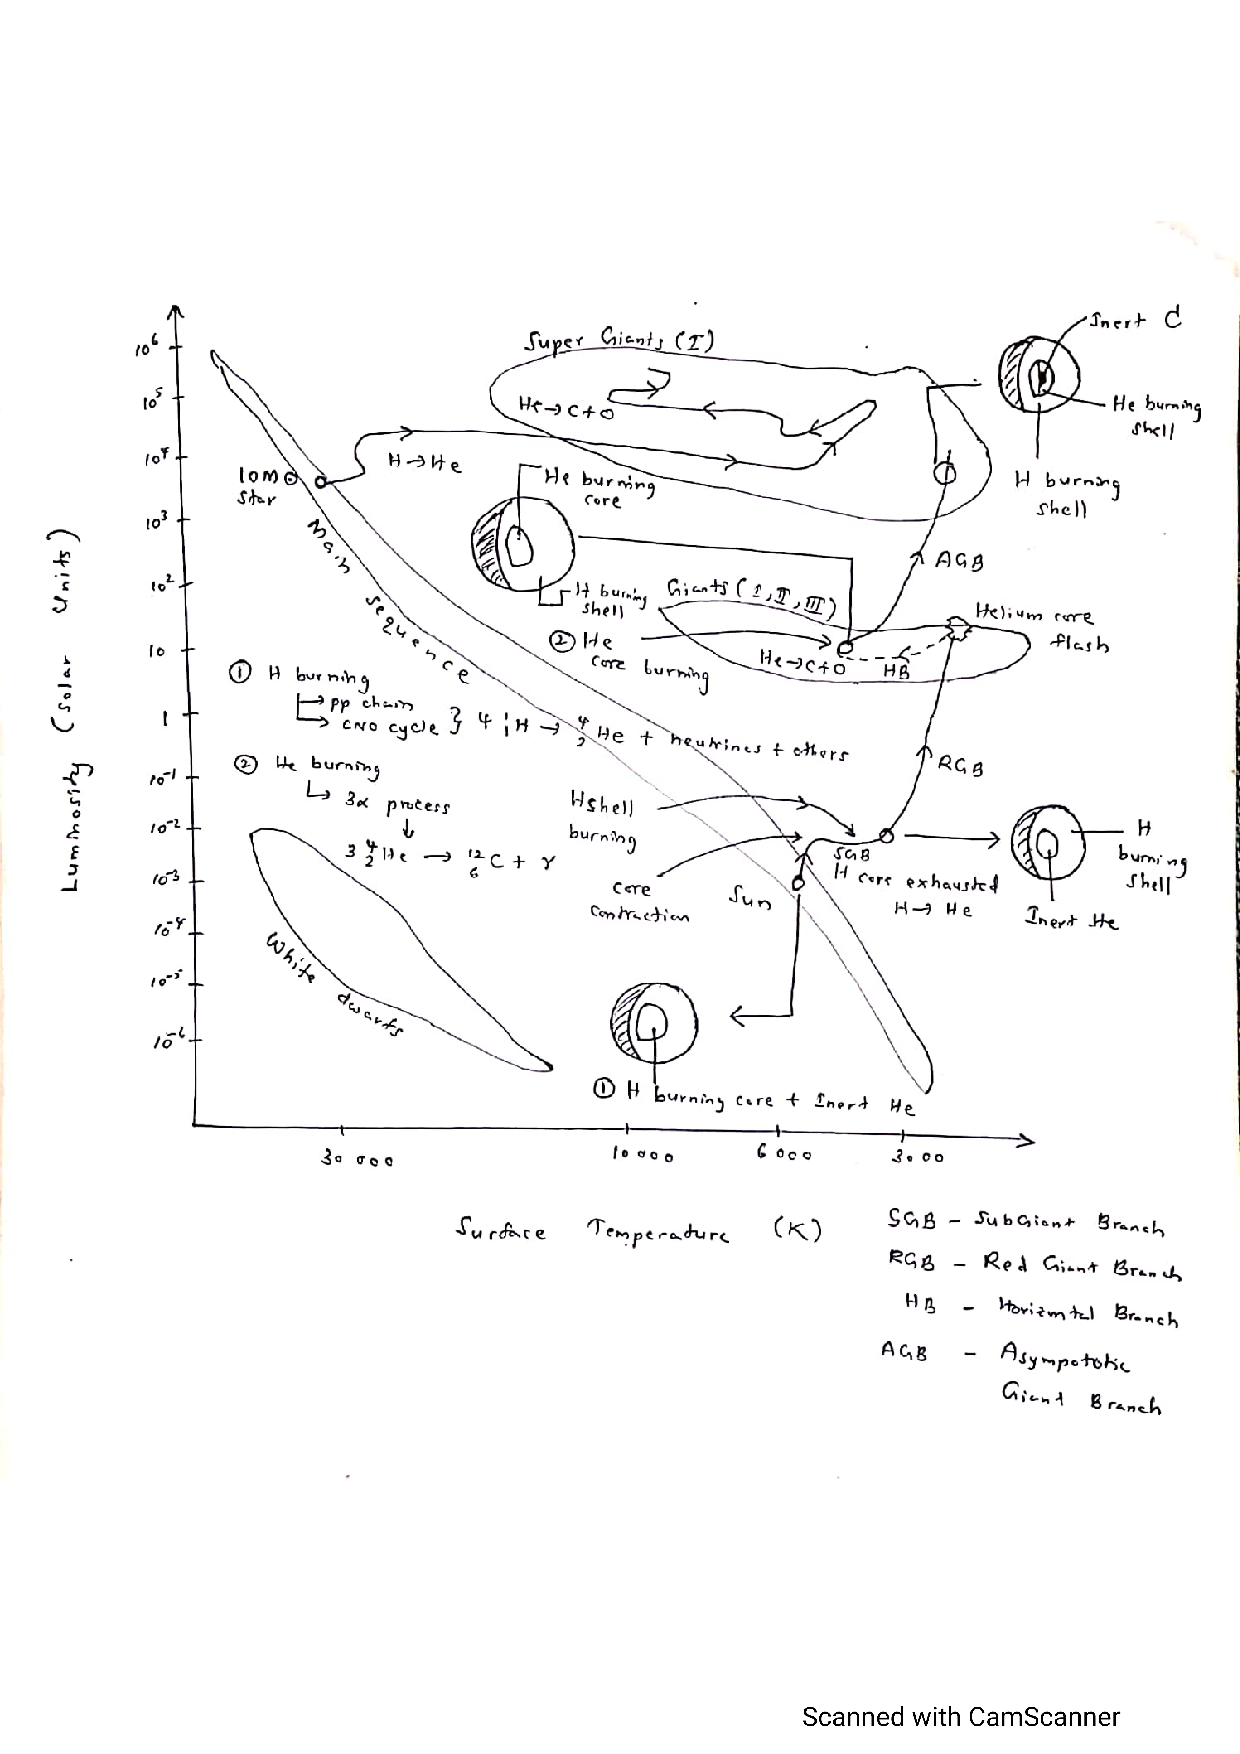
\includegraphics[width=0.9\textwidth]{Evolution.pdf}
    \caption{The simplified evolution of a star from the main sequence to the super-giant stage}
    \label{fig: PaleBlueDot}    
\end{figure}

\newpage
\paragraph*{Problem 5}
\begin{enumerate}[label=(\alph*)]
\item Where does the large amounts of energy released in supernova explosions originally come from? From nuclear processes or other processes?
\newline \textbf{Answer: }
\newline Gravitational energy is the crucial source of energy.
\item Briefly explain the conditions required to produce a core-collapse supernova explosion
\newline \textbf{Answer: }
\begin{itemize}[noitemsep,nolistsep]
%\itemsep-1em
    \item Core-collapse supernovae: Magnificent explosions that indicate the cataclysmic deaths of (defined) big stars 
    \item Reason and the process: Occurs when the iron core (iron has the highest binding-energy per nucleon, which manipulate a growing iron-nickel core under high gravitational pressure) of a massive star collapses due to the force of gravity. Once the density in the core exceeds that of nuclear matter, the core rebounds generating pressure waves that propagate outward. A shock reheating/re-energizing mechanism is needed to explode the star
    \item Conditions: The mass of the core must exceed the Chandrasekhar limit of $1.4M_\odot$. The released 'thermal' neutrinos must form as neutrino-antineutrino pairs of all flavors, and total several times the number of electron-capture neutrinos. The two neutrino production mechanisms must convert the gravitational potential energy of the collapse into a ten-second neutrino burst. The mass of the progenitor star should be below $50M_\odot$ (if not it will collapse directly into a black hole without forming a supernova explosion).
\end{itemize}
\end{enumerate}

\paragraph*{Problem 6}
\begin{enumerate}[label=(\alph*)]
\item Our Sun rotates about its axis once every 25 days. Assume that the Sun is a solid sphere and use the law of
the conservation of angular momentum to find the rotation period if the Sun is compressed to the typical size of a
white dwarf with a radius of 6000 km.
\newline \textbf{Answer: }
\newline Using the conservation of angular momentum,
\begin{equation}
    L_{before} = L_{after} \rightarrow I_1\omega_1 = I_2\omega_2\rightarrow \frac{2M_\odot R_\odot^2 \times 2\pi}{5 \times P_\odot} = \frac{2M_\star R_\star^2 \times 2\pi}{5 \times P_\star}
\end{equation}
Assuming no mass loss,
\begin{equation}
    P_\star = \frac{R_\star^2 \times P_\odot}{R_\odot^2} = \frac{6000^2 \times 25}{696340^2} = 1.856 \times 10^{-3} days
\end{equation}
\item Repeat the above calculation if the Sun is compressed to the typical size of a neutron star with a radius of 8
km.
\newline \textbf{Answer: }
\newline Assuming no mass loss,
\begin{equation}
    P_\star = \frac{R_\star^2 \times P_\odot}{R_\odot^2} = \frac{8^2 \times 25}{696340^2} = 3.300 \times 10^{-9} days
\end{equation}
\item A millisecond pulsar has period of 1 ms. What is the maximum radius that this pulsar can have before any
objects on its surface start moving faster than the speed of light?
\newline \textbf{Answer: }
\begin{equation}
    \omega = \frac{2\pi}{P} = \frac{2\pi}{10^{-3}} = 2000\pi rad/s
\end{equation}
Therefore,
\begin{equation}
    R_{max} = \frac{2.998 \times 10^8}{2000\pi} = 47.715 km
\end{equation}
\end{enumerate}

%\bibliography{references}

\end{document}

